\chapter{Simulating additive manufacturing}

\section{Present simulation approaches and challenges\label{sec:challenges}}

%\subsection{Present simulation approaches}
As a whole, AM processes are considered as an important step--change in manufacturing technologies nowadays widely used, opening up the possibility of going almost directly from Computer Aided Design to net--shape defined products. With sufficient penetration in the industrial sector, this kind of technology could have a significant impact on both the environment and on sustainable manufacturing, with large reduction of material wastage and integrated components with specific optimized features.
However, there are many challenges to be overcome to increase the importance of these technologies for the industry. These range for business considerations to technical and inherent differences in the processes from industry standards.

Computational modeling has a relatively important role to play in addressing these issues, when compared with its role in other manufacturing processes. An interesting aspect of AM from the perspective of computational modeling regards the manufacturing length scales. In a conventional casting process, for example, the local cooling rates are determined on a macroscale, thus directly linked to the size of the casting. All the phenomena occuring during such a process usually spread across a broad length scale, making a multi--scale simulation approach a rather challenging task.
On the other hand, the manufacturing length scales of powder through AM processes are much smaller and closely related to the size of the melt pool; also, solidification cooling rates are much higher. Thus, in a multi--scale simulation, the linking across the length scales could be more achievable by common modeling techniques such as finite elements or phase field simulations, both of which can guide the fabrication process to obtain components with designed features (e.g.\ microstructures, mechanical properties, etc.).

With the aid of computational modeling, there are several key areas which are subject of research interests, namely:
\begin{itemize}
    \item thermal modeling of melting and solidification;
    \item residual stress modeling;
    \item topological and shape optimization of components.
\end{itemize}

Among these topics, the first one regarding the fundamental phenomena of melting and solidification is by far the most important. Also, analysis of residual stresses has its starting point with the thermal history of the processed component.
Besides meso--scale approaches useful to bridge the gap between the modeling phase and actual industrial fabrication, also simulation techniques at the atomic scale can give valuable insights when trying to better understand complicate processes of AM.

%There are several motivations to employ atomistic simulations to study materials under the conditions they are subject to during AM processes. The foremost reason is related to the out--of--equilibrium conditions that are usually the ``scenario'' in which additive manufacturing takes place: in this context atomistic simulations are the most predictive method to investigate these aspects.

The foremost motivation to employ simulations to study the conditions materials undergo during AM processes is related to the predictive power of atomistic simulations in the context of the out--of--equilibrium scenario in which additive manufacturing takes place.

%Furthermore, there are some general physical properties that are in common with all AM techniques and atomistic simulations serve as a versatile tool to study in depth all of these properties. In this particular context, ``general'' physical properties means studying: viscosity (and the closely related diffusion coefficient), absorptance and the class of solid--liquid interface properties. We shall discuss these properties briefly in the last part of this section.

%\subsubsection{Viscosity and diffusion coefficient}
%Viscosity and diffusion coefficient are strictly related (e.g.\ by the Stoke--Einstein relation). Both of these properties are of relevant importance for AM, and especially laser--driven manufacturing: viscosity of the melt pool is required to be low enough such that it successfully spreads on the previously processed layer. According to Takamichi and Roderick, for a process like LM in which the powder system undergoes a complete melting, the dynamic viscosity of the liquid can be defined as~\cite{Takamichi1993}
%\begin{equation}
    %\eta= \frac{16}{15}\sqrt{\frac{m}{k_B T}} \gamma
    %\label{eqn:dynamic-viscosity}
%\end{equation}
%where $\gamma$ is the surface tension of the liquid (all the other quantities being self--explanatory).
%This viscosity decreases with increasing the working temperature, which in turn leads to better diffusion properties of the liquid in conjunction with solid particles and, eventually, an improved densification. An issue can be met when processing metallic system with a strong formation tendency of intermetallic compounds, which are generally brittle and may increase the viscosity of the melt.

%\subsubsection{Absorptance}
%AM processes generally involve direct interaction of metallic powders with laser beam. The study of absorptance properties of powders is particularly important because it allows one to determine the suitable ``processing window'', which, in the best case scenario, should be free of a non--response of powder due to insufficient laser energy and material evaporation due to excessive input power.
%The absorptance\footnote{It should not be confused with absorbance, which is a more specific property of matter related to the intensity of incident beam of monochromatic light and the intensity of the radiation passed through the sample: $A=\log_{10}{I_0/I}$.} is defined as the ratio of the absorbed radiation to the incident radiation. As opposed to dense materials, only a fraction of the incident radiation is absorbed by the outer surface of particles; another part of the radiation penetrates through the interparticles voids.

%Absorptance is strongly affected by and can greatly change during the laser processing; changes in thermophysical properties of powder, particle rearrangement, phase transistion and oxidation all influence absorptance. Also, absorptance is time and process dependent and generally the greater the absorptance power, the less the laser energy required.


%\subsubsection{Solid--liquid interface properties}
%Among surface properties, surface tension is by far the most relevant  when dealing with AM processes, because both in LS and LM phase transition occur and coexistence of solid and liquid is always present. The wetting behaviour of the molten system and the solidified processed layer is related to the surface tensions of solid--liquid ($\mathrm{SL}$), solid--vapour ($\mathrm{SV}$) and liquid--vapour ($\mathrm{LV}$) by the Young's equation
%\begin{equation}
    %\gamma_\mathrm{SV} - \gamma_\mathrm{SL} - \gamma_\mathrm{LV} \cos \theta_\mathrm{C}=0,
%\end{equation}
%wheren $\theta_\mathrm{C}$ is the contact angle. The main issue associated to a poor wettability of a system has been disclosed by Das~\cite{Das2003}: since metals show a rather common tendency to surface passivation with the formation of oxides, the presence of this contamination layer on the surface of melts and on previously processed layer is a strong impediment to a good wettability and causes structural defects such as balling (see \cref{sub:LM}). %One possible solution to this is carrying out AM processes under protective atmosphere, using high purity inert gases.

%Interface properties play an important role also for what regards phase transition, ubiquitous in any AM process. Studying how a phase transition occurs means being able to know what controls nucleation, which happens when the melt begins to cool down after the highly energetic interaction with the laser source, and the subsequent growth, which strongly affects the nature of the microstructure of the processed component.
%In this context, properties like the nucleation rate, the mechanism of the nucleation itself (e.g.\ planar or dendritic) and growth speed during solidification are of primary interest at the industrial level. 



%%%%%%%%%%%%%%%%%%%
%%% Open Issues %%%
%%%%%%%%%%%%%%%%%%%

%\subsection{Open issues}
%Issues related to the techniques described in previous sections can be divided in two different, though linked, fields: the first one is from a material science perspective and a second one related to technological--industrial aspects.

%General physical properties of materials that are fundamental to all laser--based manufacturing processes are absorptance, surface tension (and wettability) and viscosity: these are to be taken into account when thinking of design strategies of the target product. 

%The absorptance is defined as the ratio of the absorbed radiation to the incident radiation. AM processes generally involve a direct interaction of powders with laser beams, therefore the determination of absorptance of powders is particularly important, because it allows one to determine a suitable ``processing window'' free of a nonresponse of powder due to an insufficient laser energy input or a pronounced material evaporation due to an excessive energy input.

%Among particular properties of interests for all AM processes, there are microstructural and mechanical properties and the out of equilibrium phenomenon known as solute trapping. The first two are of primary importance for AM applications and, at the same time, they represent quite broad classes of materials properties. Solute trapping is of peculiar interest when studying solid--liquid interfaces of multi-component systems (e.g.\ ternary or more complex alloys).
%
%Mechanical properties of AM processed components are strongly linked to the solidification microstructure. The high--energy laser interaction gives rise to a very fast heating and melting of materials, which is inevitably followed by a rapid solidification on cooling. Laser--based AM processes normally offer high heating and cooling rates ($\sim\SI{100}{K/s}$)~\cite{Wright2006:GuREVIEW166} at the solid--liquid interface, producing a molten pool of quite small size ($\sim\SI{1}{mm}$)~\cite{Childs2005:GuREVIEW167}. Furthermore, the rates of quenching that occur by conduction of heat through the substrate are fast enough to produce a rapid solidification microstructure. Therefore, as a characteristic of AM processed materials, grain refinement is generally expected, due to an insufficient time for grain development and growth.
%Moreover, either chemical concentration or temperature gradients in the molten pool may generate surface tension gradient, making the solidification a non--steady state process (due to the so--called ``Gibbs--Marangoni effect''). On the other hand, rapid solidification has the kinetic limitation of crystal growth that normally follows the direction of maximum heat flow. The simultaneous but competitive action of the above two mechanisms, i.e.\ a non--equilibrium solidification nature and a localized directional growth tendency, may lead to a variety of crystal orientations with a short--range regularity~\cite{Becker2009:GuREVIEW157}. Therefore, metallic materials processed by AM may present intrinsic, more or less, anisotropic features.
%
%Another important issue concerning mechanical properties of AM--processed materials is related to the residual stresses (i.e.\ stresses that remain inside a material, when it has reached equilibrium with its environment) that arise in the parts being produced. Residual stresses may impose some serious limitations to the practical use, since they introduce part deformations and/or micro cracks. Moreover, large residual stresses can limit the load resistance of the parts compared to a stress--free state.
%
%%In general, residual stresses are considerably large in parts fabricated in a layer--by--layer fashion. A thorough theoretical and experimental study by Kruth et al.~\cite{kruth+04jmatproctech} has disclosed that the residual stress profile consists of two zones of large tensile stresses at the top and bottom of a processed part and a large zone of intermediate compressive stress in between. The magnitude and shape of the residual stress profile depend on the geometric height of the part, the material properties and laser scanning strategy and processing conditions.
%
%Among material properties the elastic modulus and the coefficient of thermal expansion play an important role in what determines the level of residual stresses.
%The elastic modulus is of primary importance when phase transformations take place, as they may be detrimental or beneficial with respect to residual stresses. Normally, the formation of brittle phases during AM may promote stress cracking, whereas some controlled phase transformations may have the potential to reduce or eliminate stresses and deformation.
%
%Laser processing conditions can be tuned to control the presence of residual stresses. For LS and LM processes, the laser scanning strategy has a significant influence on the residual stresses being developed. Normally, the stresses are larger perpendicular to the scan direction than along the scan direction~\cite{Simchi2003:GuREVIEW173}  and a  subdivision of the surface in smaller sectors has been shown to lead to a lower stress value.




\section{Focus on interfacial properties}
During first--order phase transition such as nucleation and growth, interfacial properties play a central role. In particular, the interfacial free energy between the solid and the liquid phase (usually indicated with $\gamma_{sl}$) controls the barrier for nucleation of solid in an undercooled liquid and the crystal growth, which can present different regimes: planar, cellular and dendritic, the latter of particular interest for metals.

%Despite its importance from both theoretical models and practical applications, an accurate calculation of $\gamma_{sl}$ is a rather complicated task even for the case of simple elements. Furthermore, on the experimental side, few techniques aimed at measuring this quantity are complicated by the very strict control on all experimental parameters that must be achieved to obtain accurate data.% One method, for example, involves recovering $\gamma_{sl}$ from nucleation--rate measurements: in this particular case, a major difficulty arises from the possible occurrence of heterogeneous nucleation from very low--concentration of impurities.

Several computational methods have been developed to calculate $\gamma_{sl}$, where a complete control on the experimental variables is possible. These methods are the \emph{capillary fluctuation method} (CFM), different sorts of so--called \emph{cleaving methods} (CMs) and approaches based on \emph{classical nucleation theory} (CNT). All these schemes largely rely on molecular dynamics in conjunction with Monte Carlo simulations.

%Recently, approaches of this kind coupled with the accelerated sampling technique of metadynamics have been presented: the key idea is to obtain $\gamma_{sl}$ from a free--energy map of the phase transition reconstructed by metadynamics~\cite{Angioletti-Uberti2010}, allowing also to investigate solidification and melting in out--of--equilibrium conditions~\cite{Cheng2015}, much more relevant for experiments and mesoscale models of solidification (including additive manufacturing processes).

%\subsubsection{Overview of methods}
%In the following paragraphs we try to give a quick overview of the known methods for computing the solid--liquid interfacial free energy by means of molecular simulations. We will address more attention on CFM in the next section, on which we concentrated our efforts in the present research. A thorough description of the revisited method we adopted to obtain our results will be given in Chapter~\ref{ch:CFM}.

%In CMs, bulk solid and liquid phases are separately cleaved along the surface of interest and the different phases are joined to form the interface. In this way, $\gamma_{sl}$ is obtained by measuring the work done during the process~\cite{Broughton1986,Davidchack2000PRL}.

%In the CNT approach, instead, crystalline nuclei of different sizes are introduced into a supercooled liquid phase and an orientational average of $\gamma_{sl}$ can be calculated by measuring the radius of the critical nucleus $R^*$ and inserting its value in the classical nucleation theory equation relating the critical radius and $\gamma_{sl}$
%\begin{equation}
    %R^*= \frac{2\gamma_{sl}}{\Delta G_{sl}},
%\end{equation}
%where $\Delta G_{sl}$ is the difference in Gibbs free energy between bulk solid and liquid. For small undercooling, $\Delta T$, the latter term can be approximated with $-\Delta S_f^m \Delta T$, in which $\Delta S_f^m$ is the molar entropy of fusion.

%All these methods (including CFM) have been successfully applied to model systems such as hard spheres~\cite{Broughton1986,Davidchack2006} and Lennard--Jones potential~\cite{Bai2006xs:Angioletti6,Morris2003:Angioletti10} as well as to more realistic semiempirical and quantum--mechanical systems modeled by embedded atom model (EAM)~\cite{Bai2006xs:Angioletti6} or Stillinger--Weber~\cite{Altmann1965:Angioletti7} potentials.

%Both CFM and CNT have the disadvantage of being derived with approximations valid on the macroscale and for this reason require large simulation supercells with the order of \num{e5} atoms to be applicable and give reliable results. Cleavage methods requires smaller system, but may introduce non negligible errors if the simulations performed are not completely reversible, for example if complete solidification of the liquid happends while joining it to the solid due to large relative fluctuations of the interface. Lastly, interface free energy have shown to be very sensitive to the details of the potential used. For instance, different parametrizations of EAM potentials yields values of $\gamma_{sl}$ which vary by as much as 30\%~\cite{Morris2007:Angioletti19}.









\subsection{Capillary fluctuations and free energies\label{sec:CFM}}

The capillary fluctuation method was firstly introduced by Asta and coworkers~\cite{HoytPRL2001:CFM} in 2001 and employs an analysis of height fluctuations
of the solid--liquid interface at equilibrium to extract the interface stiffness, $\sigma$.

In purely mathematical terms, the stiffness can be defined as the second--order coefficient of the power expansion of the free energy with respect to orientation. In this context, orientation means an instantaneous angle (or two of those if we deal with a 2D surface, as explained later) by which the normal of the interface is tilted with respect to the axes of the chosen coordinate system (usually a Cartesian system). From a physical point of view, the stiffness is related to the energy cost of bending the surface.

The approach of CFM has been successfully applied to derive interfacial free energies from atomistic simulations for the liquid--vapor surface of Lennard--Jones system~\cite{Sides1999:HoytREVIEW43} and for amorphous polymer films~\cite{Hapke1998:HoytREVIEW44}, just to mention a couple of examples.

The CFM starts with crystal–liquid systems that have been equilibrated at the melting point
using molecular dynamics for pure materials or Monte Carlo simulations necessary to study alloys. To minimize the number of atoms, typical simulation cells are chosen to be quasi--two dimensional, with the length of the interface $d$ much larger than the thickness of the system, $b$ (see Fig.~\ref{fig:CFM_model}). The length $d$ is chosen sufficiently large to allow measurement of capillary fluctuation amplitudes over a wide range of wavelengths.
\begin{figure}[bt]
    \centering
    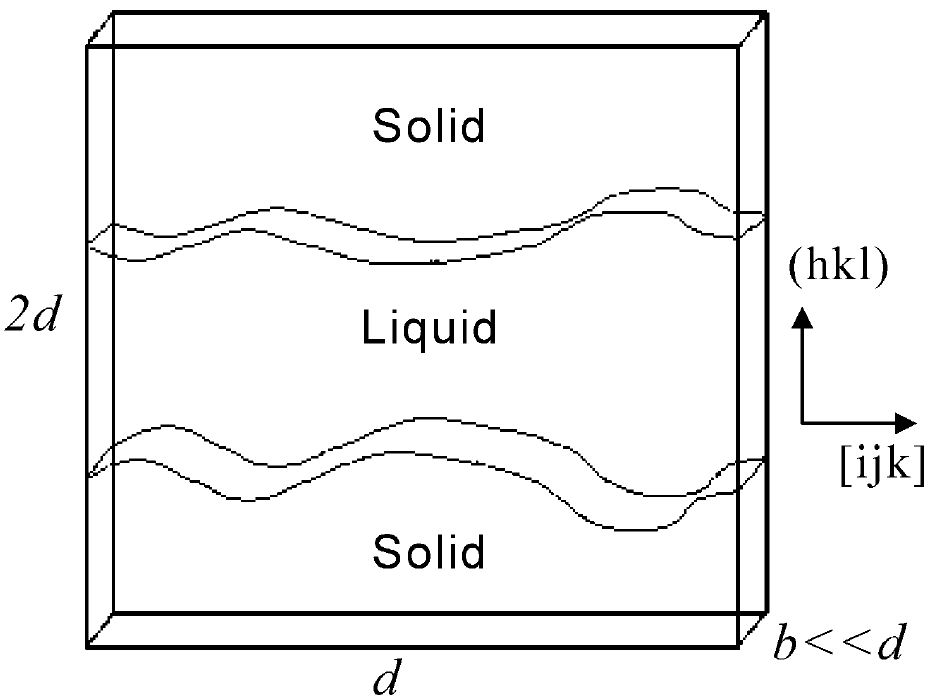
\includegraphics[width=0.5\textwidth]{CFM-model}
    \caption{Schematic model of the one dimensional system considered in the original work on the capillary fluctuation method~\cite{Hoyt2003CFMReview}.}
    \label{fig:CFM_model}
\end{figure}

Since periodic boundary conditions are applied, two identical interfaces are present in a simulation box. Thus, to avoid unwanted interactions between the two interfaces, the length of the simulation cell parallel to the interface normal is chosen to be of the order of $2d$.

In short, CFM is based upon collecting snapshots of the system during the simulation and for each of them measure the squared amplitude of capillary fluctuations. At the end of the simulation, an esemble average is computed to obtain the mean value of the amplitudes: this term is directly related to the interfacial stiffness. In this context, the stiffness $\sigma$ is defined as $\gamma + \gamma''_{\theta}$, where $\gamma''_{\theta}$ denotes the second derivative of the interfacial free energy with respect to the orientational angle $\theta$, that is the angle between the local normal to the solid--liquid interface and the average orientation for the reference flat interface. The key point of this approach is that the stiffness is one order of magnitude more anisotropic than the free energy itself, thus it can be computed more easily with smaller errors.

The CFM exploits the well--known result from capillary theory~\cite{Karma1993} for which the stiffness is directly related to the equilibrium fluctuation spectrum of a rough interface. In mathematical terms
\begin{equation}
    \langle \lvert A(k) \rvert^2 \rangle = \frac{k_B T_m}{S (\gamma + \gamma''_{\theta})k^2},
    \label{eqn:amplitudes}
\end{equation}
where $S$ is the cross sectional area of the interface and $T_m$ the melting temperature. $A(k)$ is the amplitude of an height perturbation of the interface with wavelength $\lambda=2\pi/k$ much larger than the lattice spacing. In other words, the terms denoted by $A(k)$ for different wave vectors $k$ are the coefficients of the Fourier expansion of the height function, $h(x)$
\begin{equation}
    h(x)= \sum_k A(k) \exp{(i k x)}.
    \label{eqn:fourier_expansion}
\end{equation}
The quantities $\gamma$ and $\gamma''_{\theta}$ in the denominator of Eq.~\ref{eqn:amplitudes} originate from the energy cost of bending locally the interface away from its mean orientation, which is why the fluctuation spectrum measures directly the interface stiffness.

%At this point, a fundamental question that arises is related to the method needed to construct the height function $h(x)$. To answer this question, one need to know a way of locating the interface during the simulation. To this end, the vast majority of scientific literature of CFM exploits some kind of local structural order parameter which is able to distinguish between solid and liquid atoms. Through the use of such order parameter, the position of the interface can be identified as a function of the distance along the interface (i.e.\ $x$ in this one--dimensional case, but in the most general case, one would have a function $h(x,y)$ of the two coordinates parallel to the interface). An in depth description of the way we adopted to be able to distinguish solid and liquid phases and to locate the instantaneous position of the interface will be given in the next chapter.

With \cref{eqn:amplitudes,eqn:fourier_expansion}, the CFM is used to derive values of the stiffness for several interface orientations and the results are then combined with an analytical expansion of the interface free energy $\gamma(\hat{n})$ to map out the full anisotropy of the solid--liquid interfacial free energy. For the applications considered here, the appropriate expansion for $\gamma(\hat{n})$ involves cubic harmonics, that are linear combinations of spherical harmonics that obey the cubic simmetry of the lattice. Following the approach developed by Fehlner~\cite{Fehlner1976}, the expansion for the interface free energy is
\begin{equation}
\label{eqn:cubic_harmonics}
    \frac{\gamma(\hat{n})}{\gamma_0} = 1 + \epsilon \left( \sum_{i=1}^3 n_i^4-\frac{3}{5}\right) + \delta \left( 3 \sum_{i=1}^3 n_i^{4}+ 66 n_1^2 n_2^2 n_3^2- \frac{17}{7}\right)+\cdots
\end{equation}
where $\hat{n}=(n_1,n_2,n_3)$ is the interface normal and the parameters $\epsilon$ and $\delta$ give a measure of the anisotropy of $\gamma$.

With the relation of \cref{eqn:amplitudes} and the expansion of \cref{eqn:cubic_harmonics}, three different calculations for independent interfaces are needed to obtain the parameters of the expansion ($\gamma_0$, $\epsilon$ and $\delta$). In a more recent work on dendritic growth in metals, Becker et al.~\cite{BeckerPRL2007} made use of different simulations geometries containing two--dimensional interfaces, instead of the so far discussed ``quasi'' two--dimensional. In this case, one must fully take into account the possibility of capillary waves also in the other direction parallel to the interface and the relation between amplitudes of capillary fluctuations and wave vectors becomes
\begin{equation}
    \langle \lvert A(k_x,\,k_y) \rvert^2 \rangle = \frac{k_B T_m}%
    {S( \sigma_{11}k_x^2 + \sigma_{22}k_y^2 + 2\sigma_{12}k_xk_y)}.
    \label{eqn:amplitudes_xy}
\end{equation}
2D simulation geometries require larger cells and in turn more atoms, but they present the advantage that from two independent interface normals three independent stiffness values can be obtained and so only two simulations are needed to fully parametrize $\gamma$\footnote{This follows from the fact that for two--dimensional geometries the stiffness $\sigma$ is not a scalar, but a second--order tensor with only three independent components, due to the mathematical definition of $\sigma$:\[\sigma_{ij}= \frac{\partial^2 \gamma}{\partial\theta_i\partial\theta_j}.\]%
Choosing a high symmetry interface usually imposes constraints on the stiffness tensor, reducing the effective number of independent values. For highly symmetric interfaces, only one value is kept.}. Moreover, more $k$ modes are accessible from a 2D interface, because wave vectors have the form $2\pi(j_1/L_1,\,j_2/L_2)$, where $L_1$ and $L_2$ are the lengths of the simulation box along the interface and $j_1,\,j_2$ are two non--zero indexes.


%For 2D interfaces, the stiffness $\sigma$ is a second--order tensor with three independent values in general\footnote{This is true on general grounds because of the definition of the stiffness as second--order derivative of the interface free energy with respect to the orientational angles:
%\[ \sigma_{ij}= \frac{\partial^2 \gamma}{\partial\theta_i\partial\theta_j}. \]}, but symmetry arguments can reduce the independent values for certain interface orientations.% For example, for a (100) interface in a FCC crystal, if two of the Cartesian axes are along [100] and [010] directions, the off--diagonal terms are zero and the diagonal terms are equal. In this case, the general relation of Eq.~\ref{eqn:amplitudes_xy} is similar to the equation for the 1D geometry, but it is important to stress that $\gamma$ can still be parametrized with two independent interfaces: the fact that the stiffness tensor reduces to a single component is purely a consequence of symmetry.